\cleardoublepage


\chapter{Information Extraction From Images}
\label{ch:computervision}



The task of automatically recognizing and locating objects in images and videos is of extreme importance for computers to be able to understand and interact with their surroundings. Some major applications of this particular task of object detection are pedestrian detection, surveillance, autonomous driving, text digitalization, face detection and recognition, robotics, object counting and so on \cite{Agarwal2019}. 

For this work the purpose of using object detection technologies is to convert images into text in order to allow the computer to compare an image with a moment described in text.

Feature extraction plays an important role in image classification and object detection systems which are two core components of computer vision. To put in simple terms, feature extraction is the first step in converting an image into text \cite{Tiwari2013}. Figure \ref{fig:feature_extraction} shows an example of feature extraction. However, the computer is only capable of learning that the extracted features represent a motorcycle after classifying the extracted data, which is done with the usage of pre-trained deep learning neural networks.





\begin{figure}[H]
    \centering
    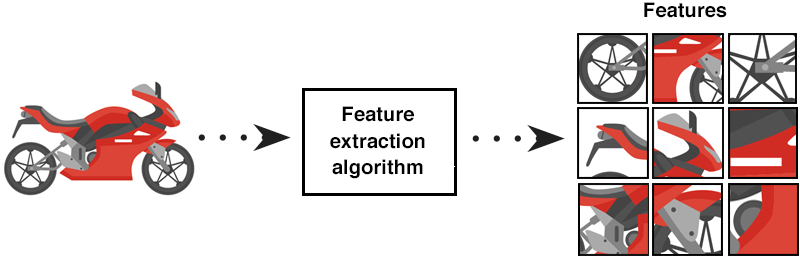
\includegraphics[scale = 0.55]{Sections/2StateOfTheArt/2_images/Feature_extraction.png}
    \caption{Feature extraction from an image. \cite{feature} }  
    \label{fig:feature_extraction}
\end{figure}


\par This chapter starts with fundamental concepts in Section \ref{sec:fundamental}. Section \ref{sec:libraries_cv} gives a brief introduction of the most common computer vision libraries. Neural networks are introduced in Section \ref{sec:neuralnet}, where the most common architecture types are presented. Finally, a state-of-the-art in object detection and image classification can be read in Section \ref{sec:state}.

\newpage

    
\section{Concepts of Label Extraction}
\label{sec:fundamental}



%%%%%%%%%%%%%%%%%%%%%%%%%%%%%%%%%%%%%%%%%%%%%%%%%%%%%%%%%%%%%%%%%%%%%%%%%%%%%

\begin{itemize}
    \item \textbf{Features and Feature Space}
\end{itemize}

    \label{sec:featurespace}
    \par A feature is considered to be a measurable piece of data in the image which is unique to a specific object, it can be color, texture or shape. Usually this features are extracted from the image and used in order to represent an object. Color is the most straightforward visual feature for indexing and image retrieval, while shape representation is the most difficult. This is because a 3-D real world object is represented in a 2-D plane in an image, which means that one dimension of information is completely lost. Texture features are very important in pattern recognition and is an important cue in region based segmentation of images.

    \par The similarity between images can be determined through features which are represented as a vector. 

    \par To sum things up, feature space is a collection of features related to some properties of the object, while a feature is an individual measurable characteristics of the object \cite{Tiwari2013}.

    %%%%%%%%%%%%%%%%%%%%%%%%%%%%%%%%%%%%%%%%%%%%%%%%%%%%%%%%%%%%%%%%%%%%%%%%%%%%%
    \begin{itemize}
        \item \textbf{Objects}
    \end{itemize}

 
    \par An object is used to identify specific items in an image or specific frames in a video. It is possible to label multiple objects in an image. An example of objects in an image of a car might be wheels, headlights, etc.
    \par Usually an object is represented by a group of features in form of a feature vector that is used to recognize objects and classify them \cite{Tiwari2013}.

    \par In object detection, small objects are normally the ones that give  worst results and lower performance when being detected. This happens because the information available to detect them is more compressed and hard to decode without some prior knowledge or context \cite{Agarwal2019}.

%%%%%%%%%%%%%%%%%%%%%%%%%%%%%%%%%%%%%%%%%%%%%%%%%%%%%%%%%%%%%%%%%%%%%%%%%%%%%%

\begin{itemize}
    \item \textbf{Image Annotation and Classification}
\end{itemize}

    Image classification is the process of associating an entire image with just one label. A simple example of image classification is labeling types of animals, cars or plants \cite{Feng2019}. \par
    Image annotation, one of the most important tasks in computer vision, is the process of annotating an image with labels. These labels are predetermined in order to give the computer vision model information about what is shown in the image, they are a combination of a bounding box in specific coordinates of the image  and a description of the object inside of it \cite{annotation}. \par

    Feeding this kind of annotated image data to a computer model teaches it to recognize the visual characteristics of that specific label, this makes the model able to categorize new unannotated images of the same type of that label. Some of these models are presented in Appendix \ref{ch:appendix}.

    \begin{itemize}
        \item \textbf{Object Detection, Segmentation and Recognition}
    \end{itemize}
    

    \par Object detection is the name given to the process that combines image classification with object localization \cite{ObjectDetection}. As previously explained, image classification is the prediction and assignment of a class label to an image, while object localization is the prediction and drawing of a bounding box around one or more objects in the image. In other words, object detection is the task that deals with the detection of objects of a certain class (e.g "flower","table","plane") in images, making it a natural extension of the classification problem. 

    \par The object detection task is considered to be a supervised learning problem, since the objective is to design an algorithm which can accurately locate and correctly classify as many instances of objects as possible, in a bounding box, while avoiding false detections in a given set of training images.  As an added challenge, many object detection applications require the problem to be solved in real time, which can be achieved. However, in order for a detector to be faster, accuracy is usually reduced. 

    \par Finally, object segmentation is the task of grouping pixels from the same object into a single region and object recognition is usually defined as giving the name of the category of an object that is contained in an image or a bounding box, assuming there is only one object in the image. For some authors object recognition can also involve detecting all objects in an image \cite{Agarwal2019}.

    A survery on classification and regression based algorithms for object detection can be read in Appendix \ref{ch:appendix}.

 

    \begin{itemize}
        \item \textbf{Image Description}
    \end{itemize}


    \par Image description is the meaning of an image and humans can understand it with relative ease. However computers only see the digital representation of images, only detecting pixels, and therefore they are not able to recognize the semantic of the image. This problem makes the semantic gap the main challenge in computer vision \cite{Huang2012}. This gap is defined by the lack of coincidence between the information extracted from visual data and the interpretation in a given situation \cite{Agarwal2019}.
    


    \par As an example, picture \ref{fig:picnic} shows an image of a family having a picnic. Feeding this image to a computer will output very different results from what a human would say.

    \begin{figure}[H]
        \centering
        \captionsetup{justification=centering}
        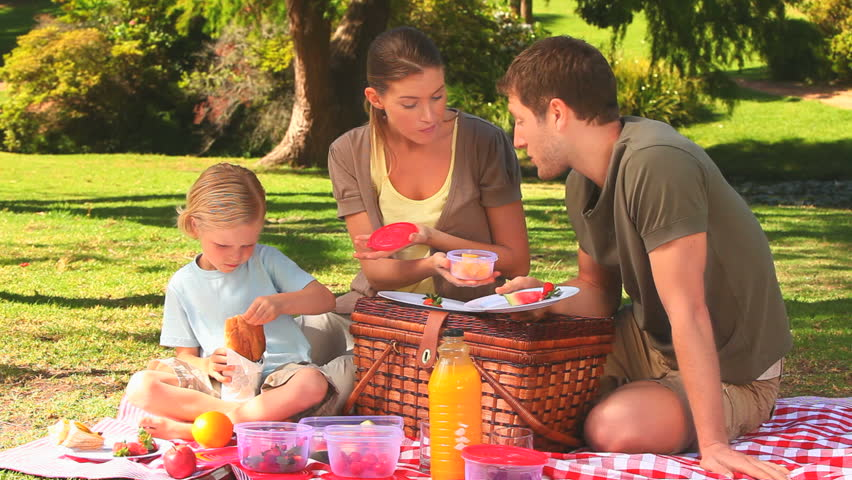
\includegraphics[width=0.5\textwidth]{Sections/2StateOfTheArt/2_images/picinic.png}
        \caption{Generic picture of a family having a picnic.}
        \label{fig:picnic}  
    \end{figure}

    Using google cloud vision API \cite{google} to extract information from the image, the following data is what the computer outputs:

    \begin{itemize}
        \item \textbf{Objects}: Person - 89\%, Person - 86\%, Person - 82\%, Tableware -59\%, Tableware - 55\%, Package goods - 54\%, Package goods - 50\%. 
        \item \textbf{Labels}: Picnic - 93\%, Recreation - 86\%, Sharing - 82\%, Event - 74\%, Summer - 70\%, Child - 61\%, Play - 57\%, Family - 52\%, Lunch - 52\%.
    \end{itemize}
   
   However, the human output would be: 
   
   \begin{itemize}
       \item \textbf{Sentence}: A family having a picnic in the park.
   \end{itemize}

     
    \par A computer is only capable of outputting the objects and labels detected but is incapable of giving them any sort of meaning like a human can.



%%%%%%%%%%%%%%%%%%%%%%%%%%%%%%%%%%%%%%%%%%%%%%%%%%%%%%%%%%%%%%%%%%%%%%%%%%%%%%


%%%%%%%%%%%%%%%%%%%%%%%%%%%%%%%%%%%%%%%%%%%%%%%%%%%%%%%%%%%%%%%%%%%%%%%%%%%%%%
    \section{Teaching a Computer on How to Learn}

    \begin{itemize}
        \item \textbf{ Artificial Intelligence }
    \end{itemize}

    Artificial Intelligence (AI) is the artificial simulation of human intelligence by a computer system in a way that it can perceive its environment, understand its behaviors and take action. Two important areas of AI are machine learning and deep learning \cite{mathworks_AI}.

    


    \begin{itemize}
        \item \textbf{Machine Learning}
    \end{itemize}
    

    \par Machine learning can be defined as a data analytics technique that allows computers to learn from experience. There are two types of machine learning techniques, which are supervised learning and unsupervised learning.
    \par Normally, supervised machine learning is used to train a model to predict future outputs, this is done by inputting and outputting known data. Supervised learning uses two different techniques which are classification and regression. Classification techniques are used to classify input data into categories while regression techniques are used to predict continuous responses. 
    \par Unsupervised learning is mostly used to find hidden patterns or intrinsic structures in input data. The most common unsupervised learning technique is clustering which is used for data analysis exploration, in order to find hidden patterns or groupings in data \cite{mathworks_ML}.

    \begin{itemize}
        \item \textbf{Deep Learning}
    \end{itemize}
    

    \par Deep Learning is a subset of Machine Learning that is inspired by the structure and function of the human brain. In order to achieve this, deep learning resorts to artificial neural networks (ANNs).
    
    \par The idea behind an ANN is that it tries to replicate the working of the human brain in the processing of data and creation of patterns, which is important for decision making. These ANNs are capable of learning unsupervised data that can either be unstructured, unlabeled or both. Putting it as simple as possible, deep learning is a machine learning technique that teaches computers to learn by example, like a human would \cite{mathworks_deeplearning}.


    \par Thanks to the new digital era, there has been an exponential increase in all forms of data, from every region of the planet. This data is defined as "big data" and comes from sources like social media, search engines, live streaming services and many others. Even though all of this information is easily accessible, it is unstructured. The problem with unstructured data is that the human brain cannot comprehend it efficiently enough to extract relevant information. However, using deep learning, all of this unstructured data can be usable.

    \par A computer model learns how to perform classification tasks directly from data, being it text, images or sound. Current deep learning models are able to achieve such levels of accuracy that they can outperform humans.

    \par In deep learning, models are trained with the usage of a large set of labeled data and neural network architectures that contain many layers. This is one of the disadvantages of deep learning, in order to improve the results of an ANN it requires to be trained with large amounts of labeled data. Since deep learning deals with such great volumes of information, this introduces another disadvantage to deep learning, which is the extreme need of higher and higher computing power.

   
        
    \par The term "deep" comes from the usage of an extensive quantity of hidden layers in the neural network. A normal neural network usually contains 2-3 hidden layers where as a deep neural network can go up to 150 hidden layers or more.

    \par As explained previously, deep learning models are trained by the usage of  large sets of labeled data and neural network architectures that are capable of automatically extracting features from the data, without the need for manual feature extraction. This automated feature extraction makes deep learning models highly accurate and practical for computer vision tasks such as object classification. 
    
    \par Deep Learning also offers "end-to-end learning", this means that a network can learn how to automatically classify raw data. In addition, deep learning algorithms scale with data, where as machine learning methods bottleneck at a certain level of performance when more examples and training data are added, which gives deep learning networks a key advantage since they improve as the size of the data increases \cite{mathworks_deeplearning}.


    The main purpose of deep learning, for this work, will be to apply it to the images provided by the imageCLEF challenge.
    
    \begin{itemize}
        \item \textbf{Computer Vision}
    \end{itemize}
    \par Computer vision is a field of artificial intelligence and computer science that aims at giving computers a visual understanding of the world \cite{cv} \cite{cv2}. It is related with pattern recognition, which is a common way to train a computer so that it can understand visual information. Pattern Recognition is the training a computer goes through when it is fed with different labeled images and then subjected to different algorithms, allowing the computer to hunt for patterns in every element related to those specific labels \cite{pattern}.


\subsection{Neural Networks}
\label{sec:neuralnet}

    \par A neural network can be considered a computer program that operates identically to how a human brain would, in the sense that it is able to be teachable to do certain tasks like problem-solving. The appeal of a neural network is the ability to emulate the human brain in pattern recognition skills. 


    \par Neural networks are composed of many small cells called neurons. These neurons are grouped into several layers that form columns. The connection between columns are formed also through their neurons. Each neuron of each layer is connected to another neuron of another layer. A visual representation of a generic neural network architecture is shown in figure \ref{fig:neural}. For further readings on neural network architectures Appendix \ref{ch:appendix} describes most of the common architectures.


    \begin{figure}[htb]
        \centering
        \includegraphics[scale = 0.5]{Sections/2StateOfTheArt/2_images/deeplearning.pdf}
        \caption{Typical neural network architecture \cite{mathworks_NN}.}
        \label{fig:neural}
    \end{figure}
        
    
    \par The connections between layers are called weighted connections and they are adjusted with a real-valued number attached to them. This number is important, because each neuron takes the value of the attached neuron (in their layer) and multiplies it by their connection weight. The bias value is an additional parameter in the neural network which is used to adjust the output along with weighted sum of the inputs to the neuron. The sum of the bias value with the weights  is put through an activation function which mathematically transforms the value and assigns it to the connected neuron in the adjacent layer. This is propagated through the whole network.  Se Figure \ref{fig:neuron} for a clear representation of this process.
    

    
    \begin{figure}[htb]
        \centering
        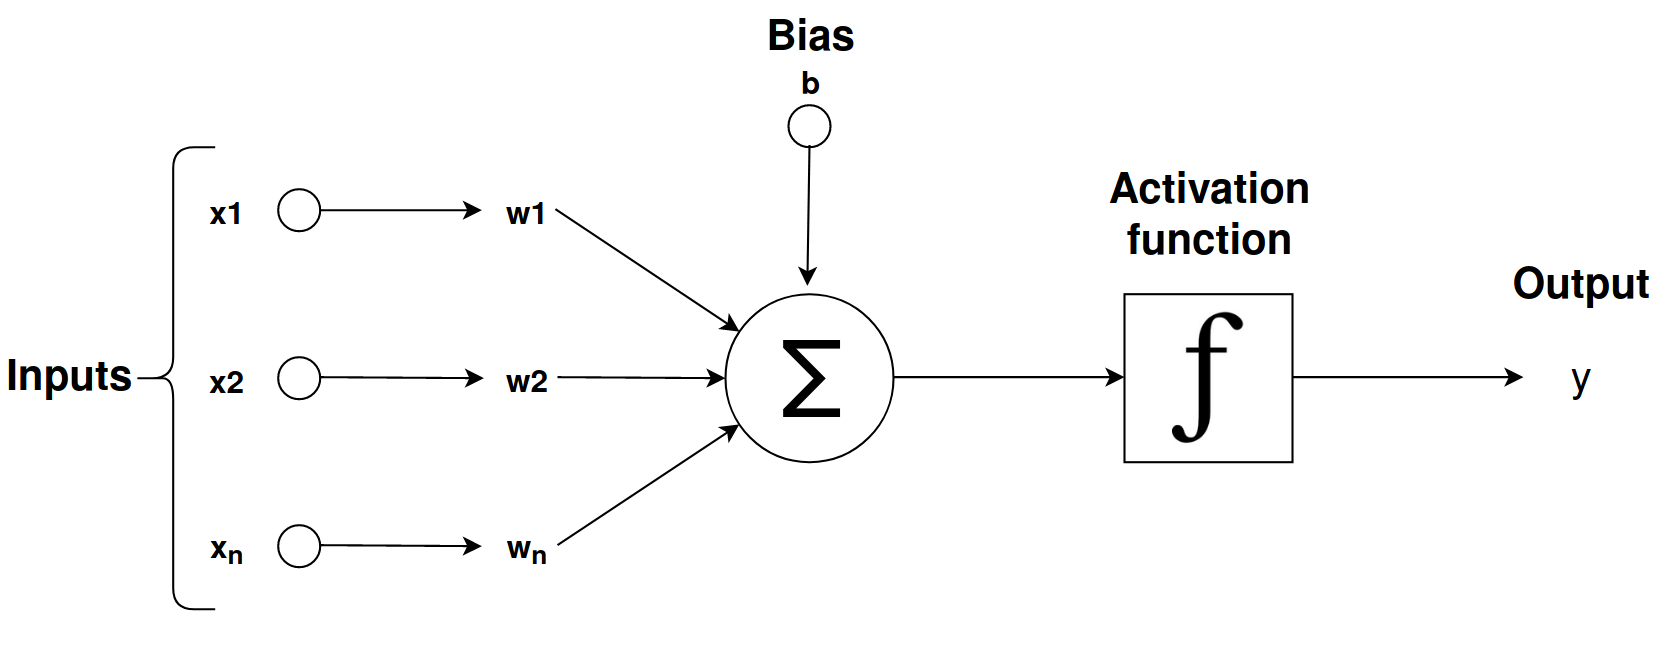
\includegraphics[scale = 0.15]{Sections/2StateOfTheArt/2_images/neuron.png}
        \caption{ Operations done by a neuron \cite{neuron}.}
        \label{fig:neuron}
    \end{figure}
    
    
   
    \par To put it simply, a neural network can be compared to a filter that goes through all of the possibilities, so that the computer is able to come up with the correct answer.
    \par Sometimes, an object might be too similar to another object which can make the network output a wrong answer. The solution to this problem is the usage of a back-propagation algorithm. This algorithm allows the network to adjust the connections back through the network, check if all the bias values are correct and all of the connections are weighted properly \cite{ArmaanMerchant2018}.
    


        \begin{itemize}
            \item \textbf{Neural Network Training}
        \end{itemize}
    \par The best way to train a neural network from scratch is to design a network architecture that will learn through the feeding of a large dataset of labeled data. This allows it it to learn the features and model. The problem with this is that depending on the learning rate of the network and the amount of data, these networks can take a lot of time to train (days, maybe weeks). 

    \par To solve the problem of time, deep learning applications can recur to the usage of transfer learning. Transfer learning is a process that involves the fine-tuning of a pretrained model. This works by using an existing network like GoogLeNet, and feed it new data of previously unknown classes to the network. After some tweaks to the network, it will be able to categorize only a specific object instead of many different ones. This not only allows the network to be more precise in categorizing that one specific object, but it will also save lot of computation time \cite{mathworks_deeplearning}.


 

%%%%%%%%%%%%%%%%%%%%%%%%%%%%%%%%%%%%%%%%%%%%%%%%%%%%%%%%%%%%%%%%%%%%%%%%%%%%%

    \section{Datasets With Common Objects}

    \label{dataset}

    \par A dataset is a collection of images and videos that contain every day life objects that are manually labeled. State-of-the-art object detection models require deep learning neural networks, and in order for neural networks to be trained, they  require training datasets, as previously explained.  

    \par A few examples of some available datasets are:  MS COCO \cite{Lin2014}, ImageNet \cite{Takamitsu1978} , VisualGenome \cite{Language2015}, OpenImages \cite{Kuznetsova2018} and Pascal-VOC \cite{Everingham2010}.

    \par Some of these datasets propose challenges, where teams are able to compete in order to achieve state-of-the-art results. This subject is discussed in section \ref{sec:state}
    %%%%%%%%%%%%%%%%%%%%%%%%%%%%%%%%%%%%%%%%%%%%%%%%%%%%%%%%%%%%%%%%%%%%%%%%%%%%%%%%%%

%%%%%%%%%%%%%%%%%%%%%%%%%%%%%%%%%%%%%%%%%%%%%%%%%%%%%%%%%%%%%%%%%%%%%%%%%%%%%


\section{Computer Vision Libraries}
\label{sec:libraries_cv}


%%%%%%%%%%%%%%%%%%%%%%%%%%%%%%%%%%%%%%%%%%%%%%%%%%%%%%%%%%%%%%%%%%%%%%%%%%%%%%%
    \begin{itemize}
        \item \textbf{OpenCV}
    \end{itemize}

    OpenCV is an open source computer vision and machine learning software library originally developed by Intel in the year 2000 \cite{Culjak2012}.\par

    The library has more than 2500 optimized algorithms, which includes a comprehensive set of both classic and state-of-the-art computer vision and machine learning algorithms. These algorithms can be used to detect and recognize faces, identify objects, classify human actions in videos, track camera movements, track moving objects, extract 3D models of objects, produce 3D point clouds from stereo cameras, stitch images together to produce a high resolution image of an entire scene, find similar images from an image database, remove red eyes from images taken using flash, follow eye movements, recognize scenery and establish markers to overlay it with augmented reality, etc. \cite{opencvweb} \par
    
    OpenCV Supports the deep learning frameworks like Tensorflow, Torch/PyTorch, Caffe and it is the most standardized tooling for computer vision.  

   \begin{itemize}
       \item \textbf{Tensorflow}
   \end{itemize} 

    \label{Tensorflow}
   

    Tensorflow is currently the most popular open source framework for numerical computation and large-scale machine learning introduced by google and was originally created for tasks with heavy numerical computations.  \cite{Abadi} \cite{Dignam1983} 
    
    Tensorflow is written in c++ which enables extremely fast compile times, non the less, it can still be accessed by other languages, such as Python and also supports CPUs, GPUs and distributed processing. \par
    

    The name given to tensorflow comes from the inputs, since it receives inputs as a multi-dimensional array, also known as tensors. The input (tensor) goes on one end and then it “flows” throughout a system of operations and comes out on the other end as output. \par 
    
    Tensorboard is a feature of tensorflow that allows the monitoring of what tensorflow is doing graphical and visually.\par

%%%%%%%%%%%%%%%%%%%%%%%%%%%%%%%%%%%%%%%%%%%%%%%%%%%%%%%%%%%%%%%%%%%%%%%%%%%%%  
    \begin{itemize}
        \item \textbf{VLFeat}
    \end{itemize}

    The VLFeat open source library implements popular computer vision algorithms specializing in image understanding and local features extraction and matching. Algorithms include Fisher Vector, VLAD, SIFT, MSER, k-means, hierarchical k-means, agglomerative information bottleneck, SLIC superpixels, quick shift superpixels, large scale SVM training, and many others. It is written in C for efficiency and compatibility, with interfaces in MATLAB for ease of use, and detailed documentation throughout. It supports Windows, Mac OS X, and Linux \cite{vedaldi08vlfeat}.

    \begin{itemize}
        \item \textbf{BoofCV}
    \end{itemize}

    BoofCV is an open source library written from scratch for real-time computer vision. Its functionality covers a range of subjects, low-level image processing, camera calibration, feature detection/tracking, structure-from-motion, fiducial detection, and recognition. \par
	This library is organized into several packages: image processing, features, geometric vision, calibration, recognition,visualize, and IO. Image processing contains commonly used image processing functions which operate directly on pixels. Features contains feature extraction algorithms for use in higher level operations. \par Calibration has routines for determining the camera's intrinsic and extrinsic parameters. Recognition is for recognition and tracking complex visual objects. Geometric vision is composed of routines for processing extracted image features using 2D and 3D geometry. Visualize has routines for rendering and displaying extracted features. IO has input and output routines for different data structures \cite{boofcvweb}.

    \begin{itemize}
        \item \textbf{GluonCV}
    \end{itemize}

    GluonCV is a toolkit that offers pre-trained models, performance metrics of the different available models, consistent interface for when switching between the models, regular re-training and continuous integration to ensure code correctness, detailed documentation and well-documented examples. It also supports a range of different applications like : image classification, object detection, semantic segmentation, instance segmentation, pose estimation, video action recognition, depth prediction and a few others.

   In short, gluonCV provides implementations of state-of-the-art deep learning algorithms in computer vision. It aims to help engineers, researchers, and students quickly prototype products, validate new ideas and learn computer vision \cite{Guo2019}.

    
%%%%%%%%%%%%%%%%%%%%%%%%%%%%%%%%%%%%%%%%%%%%%%%%%%%%%%%%%%%%%%%%%%%%%%%%%

    


\section{Recent Innovations and Improvements}
\label{sec:state}

\par Image classification and object detection are both subjects that are constantly innovating and improving upon previously results, every month new papers are published with new and more efficient networks. 
\par In the Figures \ref{fig:leaderboard_object} and \ref{fig:leaderboard_image} it is shown  not only the current best methods for both image classification and object detection but also the development of the state-of-the-art throughout the years.


\begin{figure}[H]
    \centering
    \captionsetup{justification=centering}
    \begin{subfigure}{0.49\textwidth}
        \includegraphics[width=\textwidth]{Sections/2StateOfTheArt/2_images/chart_object.pdf}
        \caption{Object Detection on COCO test-dev benchmark \cite{papers_object}}
        \label{fig:leaderboard_object}
        \end{subfigure}
        \begin{subfigure}{0.49\textwidth}
        \includegraphics[width=\textwidth]{Sections/2StateOfTheArt/2_images/chart_image.pdf}
        \caption{Image Classification on ImageNet benchmark \cite{papers_image}}
        \label{fig:leaderboard_image}
        \end{subfigure}
    \label{fig:example_f1}
\end{figure}




\par Due to the fact that object detection is a subject of great innovation, there is an extreme amount of papers that try to compete for the best results coming out every few months. So, in order to do a review of the state-of-the-art, the Tables \ref{table:cocotable} and \ref{table:imagenettable} show the benchmarks for both imageNet and COCO test-dev. These tables were obtained from \cite{Ribeiro} and are based on the analysis of \cite{papers_image} and \cite{papers_object} which is a website dedicated to  the current state-of-the-art for object detection and image classification.






\subsection{COCO Test-Dev}

\par The COCO benchmark \cite{Lin2014} is a dataset that places object recognition in the context of scene understanding. The evaluation metric used is the average precision (AP). Table \ref{table:cocotable} shows the current best architectures and their respective score for the COCO test-dev dataset.

\begin{table}[H]
    
    \centering
    \caption {COCO Test-Dev Benchmarks.}
    \begin{tabular}{| c | c | c | c ||} 
    \hline
    Method & Backbone & AP (\%)  \\ [0.5ex] 
    \hline\hline
    Liu et al.(2019) \cite{Liu2019}  & ResNeXt-152 & 53.3 \\ 
    \hline
    Tan et al. (2019) \cite{Tan2019} & EfficientNet & 51.0 \\
    \hline
    Zhang et al. (2019) \cite{Zhang2019} & ResNeXt-101 & 50.7
    \\
    \hline
    Girshick et al. (2018) \cite{Detectron2018} & ResNeXt-152 & 50.2
    \\
    \hline
    Li et al. (2019) \cite{Li2019} & ResNet-101 & 48.4
    \\ [1ex] 
    \hline
    Zhang et al. (2019) \cite{Zhang2019} & ResNet-101  & 46.3
    \\ [1ex]
    \hline
    Mahajan et al. (2018) \cite{Mahajan2018} & ResNeXt & 45.2
    \\ [1ex]
    \hline
    Zhao et al. (2019) \cite{Zhao2019} & VGG16 & 44.2
    \\ [1ex]
    \hline
    Cai et al. (2018) \cite{Cai2018} & ResNet-101 & 42.8
    \\ [1ex]
    \hline
    Wang et al. (2019) \cite{Wang2019} & ResNet-50    & 39.8
    \\ [1ex]
    \hline
    Lin et al. (2017) \cite{Lin2017} & ResNet-101 & 39.1
    \\ [1ex]
    \hline
    Shrivastava et al. (2016) \cite{shrivastava2016skip} & Inception-ResNet-v2 & 36.8
    \\ [1ex]
    \hline
    Kim et al. (2018) \cite{Kim2018} & VGG-16 & 35.2
    \\ [1ex]
    \hline
   \end{tabular}
   \label{table:cocotable}
\end{table}

\par Liu et al. \cite{Liu2019} achieved the best score in the COCO Test-Dev in 2019. They proposed better detection performance by creating a more powerful backbone network from previously existing backbones like ResNet \cite{He2016} and ResNetXt \cite{Xie2017}. They implemented a strategy for assembling multiple identical backbones (called Assistant Backbones and Lead Backbones) linked by composite connections between the adjacent backbones in order to form a more powerful backbone which was given the name of Composite Backbone Network (CBNet).

\par In typical CNN based detectors, the backbone network (the baseline of a network architecture) is used for basic feature extraction.

\par CBNet feeds the output features of the previous backbone as an input feature to the succeeding backbone through composite connections.At the final stage, the Lead Backbone outputs features for object detection.

\par This architecture was able to achieve the best result in the COCO Test-Dev with a 53.3\% AP with single model by integrating a CBNet using triple ResNeXt-152 \cite{Xie2017} backbones into the Cascade Mask R-CNN baseline.


\par Figure \ref{fig:cbnet} presents the architecture for CBNet.



\begin{figure}[H]
    \centering
    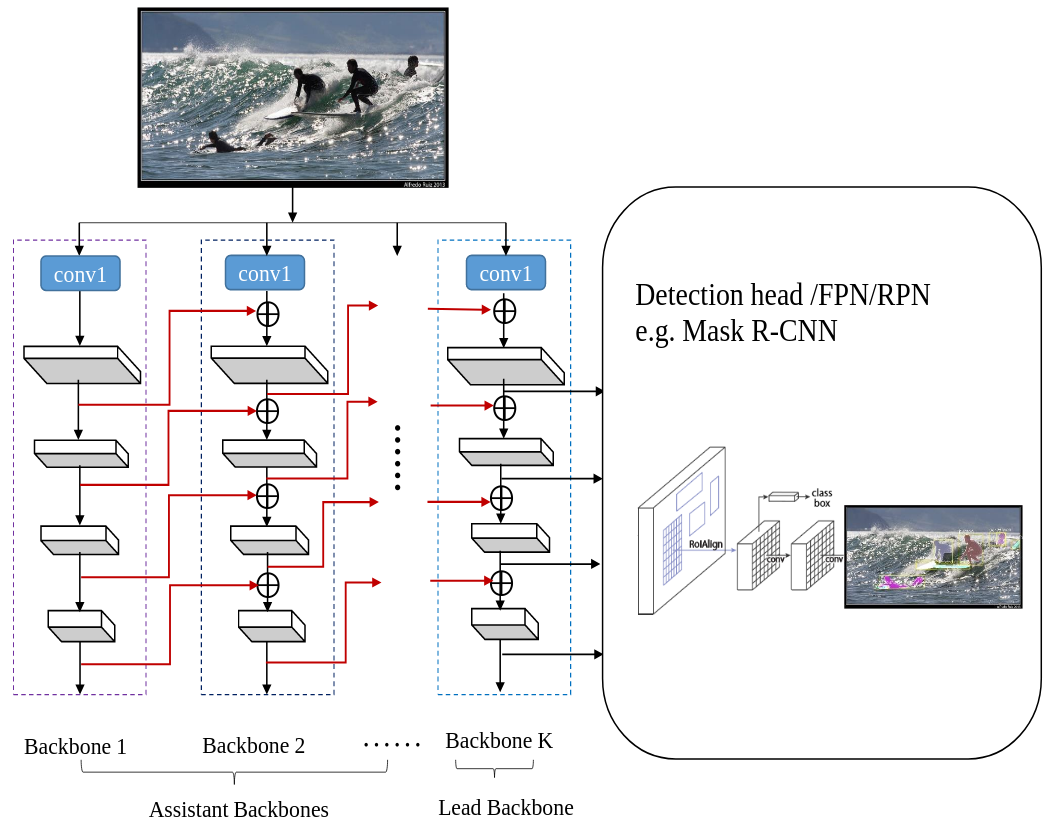
\includegraphics[scale = 0.25]{Sections/2StateOfTheArt/2_images/cbnet.png}
    \caption{CBNet Architecture for object detection \cite{Liu2019}.} 
    \label{fig:cbnet}
\end{figure}


\begin{itemize}
    \item \textbf{ResNeXt}
\end{itemize}

\label{sec:resnext}
\par ResNeXt, also known as Aggregated Residual Transform Network was created by facebook researchers and it is a simple highly modularized network architecture for image classification. 
\par The network is constructed by repeating a building block that aggregates a set of transformations with the same topology. The simple design results in a homogeneous, multi-branch architecture that has only a few hyper-parameters to set. This strategy creates a new dimension, which was given the name of "cardinality" (size of the set of transformations). 
\par This architecture is an improvement over the Inception architectures, being more simple in design and adding more branches (towers) within modules. \cite{Xie2017}


\begin{figure}[htb]
    \centering
    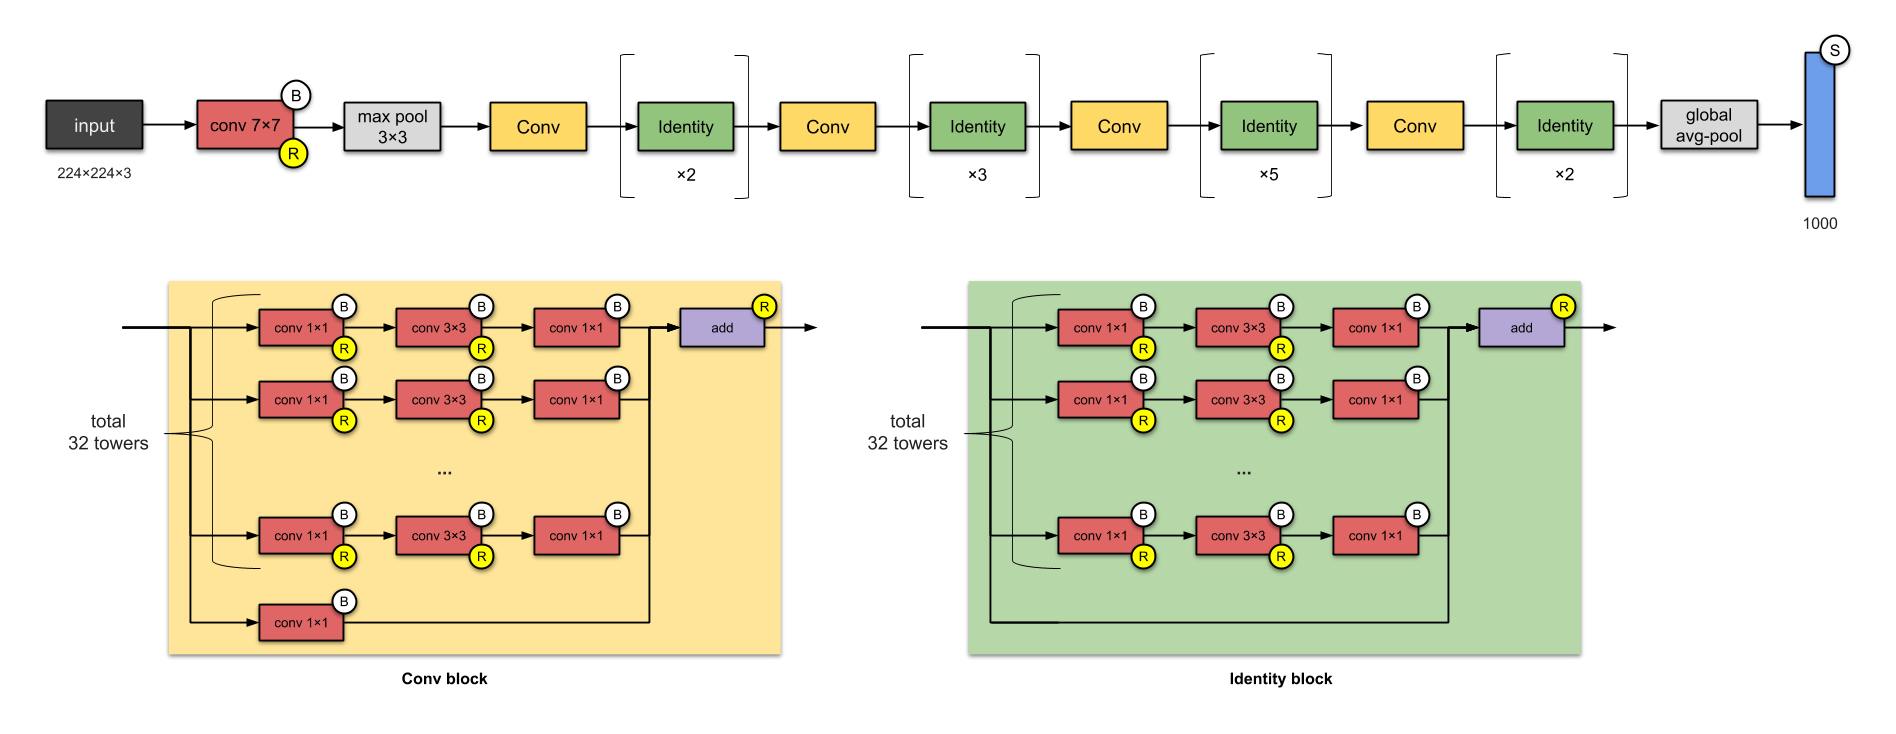
\includegraphics[scale = 0.23]{Sections/2StateOfTheArt/2_images/resnext.png}
    \caption{ResNeXt architecture \cite{cnnarchitectures}. }
    \label{fig:noisestudent}
\end{figure}


\newpage

\subsection{ImageNet}
\par The imageNet Large Scale Visual Recognition challenge \cite{Russakovsky2015} is a benchmark for object category classification and detection. The evaluation metrics used are top-1 and top-5 accuracy.

\begin{table}[htb]
    
    \centering
    \caption {ImageNet Benchmarks.}
    \begin{tabular}{|| c | c | c ||} 
    \hline
    Method & Backbone & Top-1 Acc (\%)  \\ [0.5ex] 
    \hline\hline
    Xie et al. (2019) \cite{Xie2019}& EfficientNet & 88.4
    \\ 
    \hline
    Kolesnikov et al. (2019) \cite{alex2019large} & ResNet-152 & 87.8

    \\
    \hline
    Touvron et al. (2019) \cite{touvron2019fixing} & ResNeXt-101 & 86.4

    \\
    \hline
    Xie et al. (2019) \cite{xie2019adversarial} & EfficientNet & 85.5

    \\ [1ex] 
    \hline
    Mahajan et al. (2018) \cite{Mahajan2018} & ResNeXt & 85.4

    \\ [1ex]
    \hline
    Tan et al. (2019) \cite{tan2019efficientnet}& EfficientNet & 84.4

    \\ [1ex]
    \hline
    Touvron et al. (2019) \cite{touvron2019fixing} & ResNet-50 & 82.5

    \\ [1ex]
    \hline
    Szegedy et al. (2017) \cite{szegedy2016inceptionv4} & Inception-resnet-v2 & 80.1

    \\ [1ex]
    \hline
    Szegedy et al. (2017) \cite{szegedy2016inceptionv4}  & Inception-v4 & 80.0

    \\ [1ex]
    \hline
    Simonyan et al. (2014) \cite{simonyan2014deep} & VGG-16 & 74.4
    \\ [1ex]
    \hline
   \end{tabular}
   \label{table:imagenettable}
\end{table}



\par Xie et al. \cite{Xie2019} stated that current state-of-the-art vision models are still trained with supervised learning, which implies the necessity of large corpus of labeled images in order to work properly. The fact that current models are only shown labeled images causes an obvious limitations in the improvement of accuracy and robustness of current state-of-the-art models, this can be improved with the usage of the large available quantities of unlabeled images available.
\par Having this in mind, they decided to use unlabeled images to improve the state-of-the-art ImageNet accuracy and show that accuracy has an outsized impact on robustness. For this purpose, they used a much larger corpus of unlabeled images, where a large fraction of images did not belong to ImageNet training set distribution.
\par Using a self-training framework the model was trained with 3 main steps which consist in:

\begin{enumerate}
    \item Training of a teacher model on labeled images.
    \item Usage of the teacher to generate pseudo labels on unlabeled images.
    \item Train a student model on the combination of labeled images.
\end{enumerate}

\par The algorithm was iterated a few times by treating the student as a teacher to relabel the unlabeled data and training a new student.

\par An important discovery was made during the training of the algorithm. For the method to work well at scale the student model should be noised during its training while the teacher should not be noised during the generation of pseudo labels. This way, the pseudo labels are as accurate as possible and the noised student is forced to learn harder from the pseudo labels. To induce noise in the model it was used RandAugment data, dropout and stochastic depth during the training. Figure \ref{fig:noisestudent} shows a brief view of how the method works.
\par This is where the name of the method "Noisy Student"comes from, since the student is noised to learn beyond the teacher's knowledge.
\par With this method they were able to show that it is possible to use unlabeled images to significantly advance both accuracy and robustness of state-of-the-art imageNet models.
\par The presented model uses EfficientNe as a backbone trained on images from imageNet dataset and was able to obtain the best results in the ImageNet benchmark dataset by achieving an accuracy of 88.4\%.



\begin{figure}[htb]
    \centering
    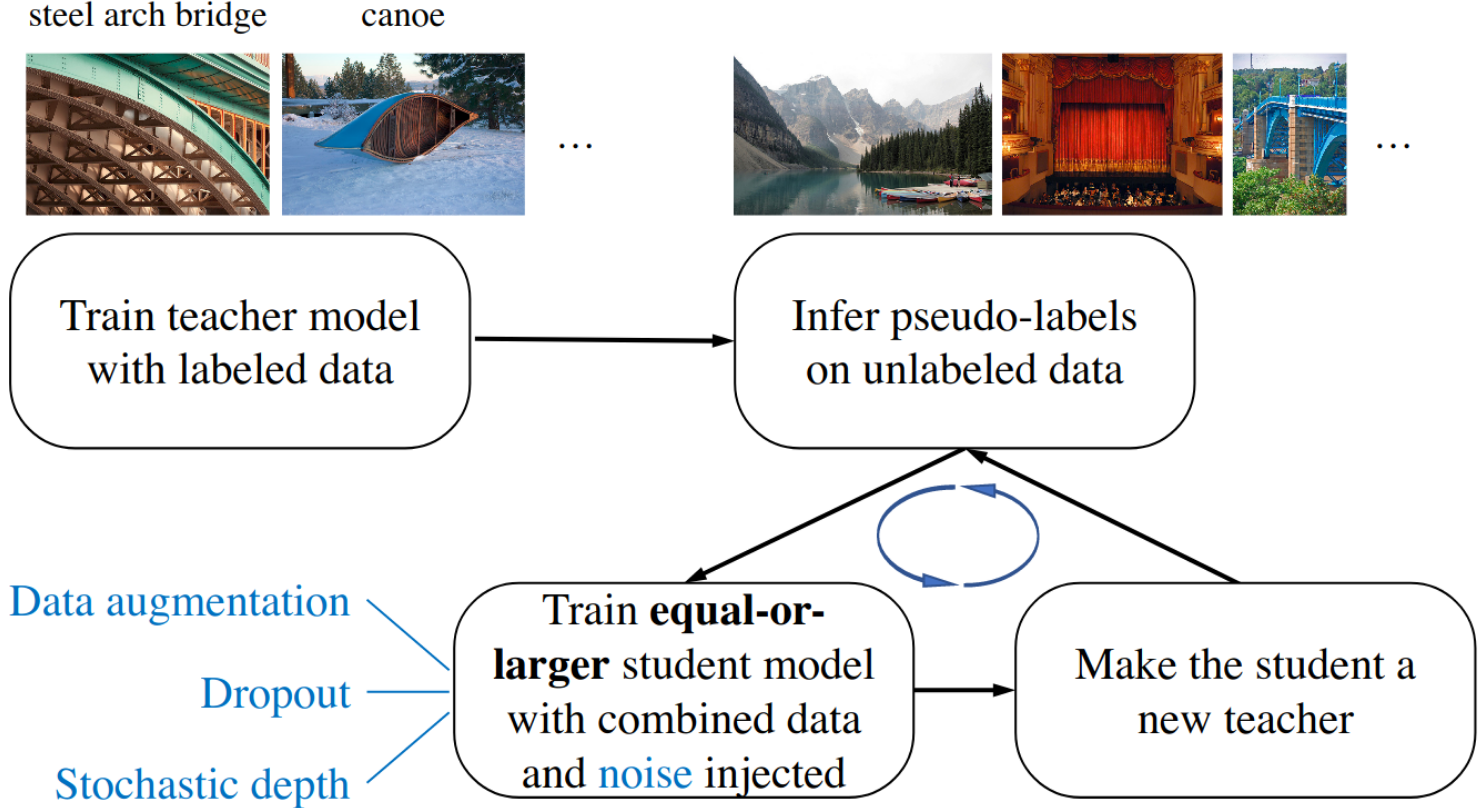
\includegraphics[scale = 0.15]{Sections/2StateOfTheArt/2_images/noisy_student.png}
    \caption{Noisy Student Method \cite{Xie2019}.} 
    \label{fig:noisestudent}
\end{figure}cnnarchitectures

\par Researchers at Google decided to study the impact of scaling up CNNs, in order to achieve better accuracy and efficiency. EfficientNet-B0 was developed based on a simple idea, scaling each of the dimensions of the network (width, depth and resolution) with a constant ratio, improves the overall performance \cite{tan2019efficientnet}.

\begin{figure}[htb]
    \centering
    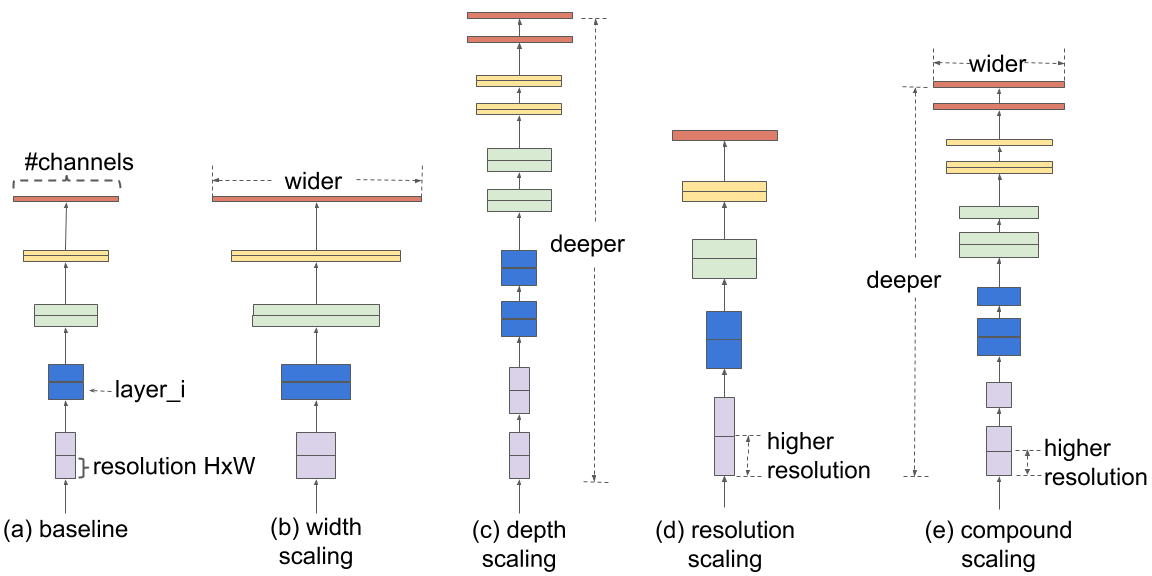
\includegraphics[scale = 0.25]{Sections/2StateOfTheArt/2_images/efficientNet_scale.png}
    \caption{Comparison of different scaling methods:  (a) is a baseline network example; (b)-(d) are conventional scaling that only increases one dimension of network  width, depth, or resolution. (e) is the proposed compound scaling method that uniformly scales all three dimensions with a fixed ratio \cite{tan2019efficientnet}.
    } 

\end{figure}

\newpage

\par The baseline network architecture, EffecientNet-B0, uses mobile inverted bottleneck convolution (MBConv), similar to MobileNetV2 \cite{s2018mobilenetv2} and MnasNet \cite{tan2018mnasnet}. Figure \ref{fig:eff} shows the baseline network architecture EfficientNet-B0.

\begin{figure}[htb]
    \centering
    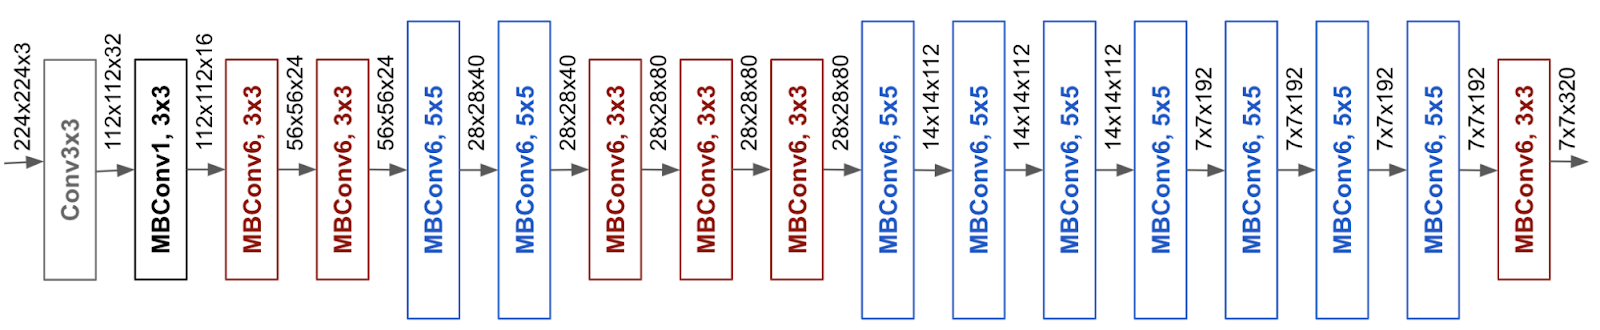
\includegraphics[scale = 0.22]{Sections/2StateOfTheArt/2_images/efficientNet_Arch.png}
    \caption{EfficientNet-B0 architecture representation \cite{Tan}.} 
    \label{fig:eff}

\end{figure}


\section{Final Remarks}


The models and algorithms experimented in this thesis were provided trough a computer vision python library called imageAI, which allows the ability to easily use state-of-the-art AI features \cite{ImageAI}. This library required the pre-installation of TensorFlow, OpenCV and Keras libraries. The Keras library \cite{CholletFrancois2015} is an open-source neural-network library written in Python which is capable of running on top of TensorFlow.

During the development of the automatic retrieval system many of the described algorithms and models in Appendix \ref{ch:appendix} were tried. For image classification the algorithms tested were DenseNet, InceptionV3, ResNet and SqueezeNet. For object detection the models used were YoloV3, TinyYoloV3, RetinaNet and ResNetXt-101. The testing of all of these models was done in order to find the most suitable model to process the imageCLEF images dataset.